\documentclass{beamer}

\usepackage[utf8]{inputenc}
\usepackage[russian]{babel}  % Russian layout
\usepackage{amsmath,mathrsfs,amsfonts,amssymb}
\usepackage{graphicx, epsfig}
\usepackage{subfig}
\usepackage{floatflt}
\usepackage{comment}
\usepackage{epic,ecltree}
\usepackage{mathtext}
\usepackage{fancybox}
\usepackage{fancyhdr}
\usepackage{enumerate}
\usepackage{epstopdf}
\usepackage{Iv_commands}

\DeclareMathOperator{\argmin}{arg\!min}
\DeclareMathOperator{\argmax}{arg\!max}

\usetheme{Frankfurt}%{Singapore}%{Warsaw}%{Warsaw}%{Darmstadt}%{Frankfurt}%{Dresden}
\definecolor{beamer@blendedblue}{RGB}{15,120,80}
\definecolor{light-gray}{rgb}{0.8,0.8,0.8}

\setbeamercolor{frametitle}{fg=Brown,bg=Brown!20}
\setbeamercolor{section in head/foot}{bg=Brown}
\setbeamercolor{author in head/foot}{bg=Brown}
\setbeamercolor{date in head/foot}{fg=Brown}

\usecolortheme{sidebartab}
\useinnertheme{circles}
%----------------------------------------------------------------------------------------------------------
\title[\hbox to 56mm{\hfill\insertframenumber\,/\,\inserttotalframenumber}]
{Мультимоделирование SVM}
\author[С. Иванычев, А. Адуенко]{\large \\Сергей Иванычев, Александр Адуенко}
\institute[МФТИ]{Московский физико-технический институт \\
    Факультет управления и прикладной математики\\
    Кафедра <<Интеллектуальные системы>>
}
\date{\footnotesize{}}
%----------------------------------------------------------------------------------------------------------
\begin{document}
%----------------------------------------------------------------------------------------------------------

\begin{frame}
%\thispagestyle{empty}
\titlepage
\end{frame}
%-----------------------------------------------------------------------------------------------------
\begin{frame}{Цель исследования}
Отобрать оптимальный набор ядер и построить на них композицию SVM. Описать
отличия множеств опорных объектов, генерируемые разными ядрами.


     \begin{block}{Проблемы}
        Существующие методы комбинирования алгоритмов плохо работают с малым количеством сильных классификаторов\\
        Различные ядра могут в реальности быть ``похожими'' и давать схожие результаты,
        их нецелесообразно использовать в композиции. 
    \end{block}
    \begin{block}{Предположение}
        Можно использовать вектора отступов как новые объекты и построить классификатор над ними. Схожесть ядер можно описать с помощью новой метрики, основанной на множествах опорных объектов. 
    \end{block}
\end{frame}
%----------------------------------------------------------------------------------------------------------
\begin{frame}{Литература}
    \begin{enumerate}
        \footnotesize {
        \item
            Rauf Izmailov, Vladimir Vapnik and Akshay Vashist. Multidimensional Splines with Infinite Number of Knots as SVM Kernels. 2013
        \item
            Alex J Smola et al. A Tutorial on Support Vector Regression. 2004
        \item
            Corinna Cortes and Vladimir Vapnik. Support-Vector Networks. 1995
            }
     \end{enumerate}
\end{frame}
% %----------------------------------------------------------------------------------------------------------
\begin{frame}{Постановка задачи}
    
        $X^l = (\mathbf{x}_i, y_i)_{i=1}^l$ --- обучающая выборка, $\mathcal{K} = \{K_i\}_{j=1}^m$ --- множество ядер. 
    \begin{block}{Определение}
        \textbf{Модель} с порядковым номером $s$ --- SVM c ядром $K_s \in \mathcal{K}$
    \end{block}

    Совокупность моделей генерирует для обучающей выборки матрицу $M \in \mathbb{R}^{l \times m}$, где $(i, j)$-й элемент --- отступ $i$-го объекта на $j$-й модели.
    $M$ --- новая матрица ``\emph{объект-признак}''

    Пусть $\mathcal{A}$ ---~ множество алгоритмов вида
$$
    \mathcal{A} = \fbrs{a(\vec{x}) = g(\vec{x}, \theta)|\theta \in \Theta}\;\; g:\R^m \to Y
$$

\end{frame}
% %----------------------------------------------------------------------------------------------------------

\begin{frame}{Постановка задачи}

    \begin{block}{Определение}
        Мультимодель --- пара $(g, \mathcal{K'})$, где $\mathcal{K'} \subset \mathcal{K}$
    \end{block}
Тогда перед нами стоит задача отбора ядер из $\mathcal{K}$ (то есть задача
отбора признаков из $M$) и а также выбор оптимального алгоритма для аггрегации
множества моделей в мультимодель с лучшим качеством классификации и регрессии.
$$
    L(y, g(M, \theta)) \to \min_{\mathcal{A}, \Theta}
$$
\end{frame}

% ==============================================================================

\begin{frame}{Цели эксперимента}

Необходимо найти способ определять схожие модели, то есть дающие схожие результаты, 
 чтобы не включать таковые в мультимодель. 

\begin{block}{Гипотеза}
    Если множества опорных объектов пары классификаторов похожи
    , то и векторы отступов похожи.
\end{block}

\begin{block}{Цель эксперимента}
    Сформулировать понятие ``похожести'' веторов отступов
    и различных моделей и проверить гипотезу.
\end{block}



\end{frame}
% ==============================================================================
\begin{frame}{Эксперимент. Ядра и данные.}

В качестве исходных данных взяты датасеты German Credits, Wine и Heart disease из UCI.

Ядра:

\begin{itemize}
    \item Линейное
    \item Полиномиальное (степени 3, 4, 5)
    \item RBF-ядро ($\gamma \in \{0.0001, 0.001, 0.01, 0.1, 1\}$)
    \item {\color{red} INK-spline ядро}
\end{itemize}

    
\end{frame}
% ==============================================================================
\begin{frame}{Эксперимент. Метрики}

Расстояние между ядрами представим в виде нормализованной симметрической разности:

\begin{block}{}
    $$
\rho_{X^l}(K_i, K_j) = \frac{\#\sbrs{\mathrm{SV}_i \;\Delta\; \mathrm{SV}_j}}
{\#\sbrs{\mathrm{SV}_i \cup \mathrm{SV}_j}}
    $$
\end{block}

В качестве меры сходства классификаторов возьмем отнормированную корреляцию Пирсона векторов отступов.

\begin{block}{}
    $$
\rho_{X^l}(M_i, M_j) = 1 - \mathrm{corr}(M_i, M_j)
    $$
\end{block}

Проанализируем эволюцию распределения пар расстояний в зависимости от параметра регуляризации.
    
\end{frame}

% ==============================================================================
\begin{frame}{Эксперимент. German credit}

\begin{figure}[H]
      \center{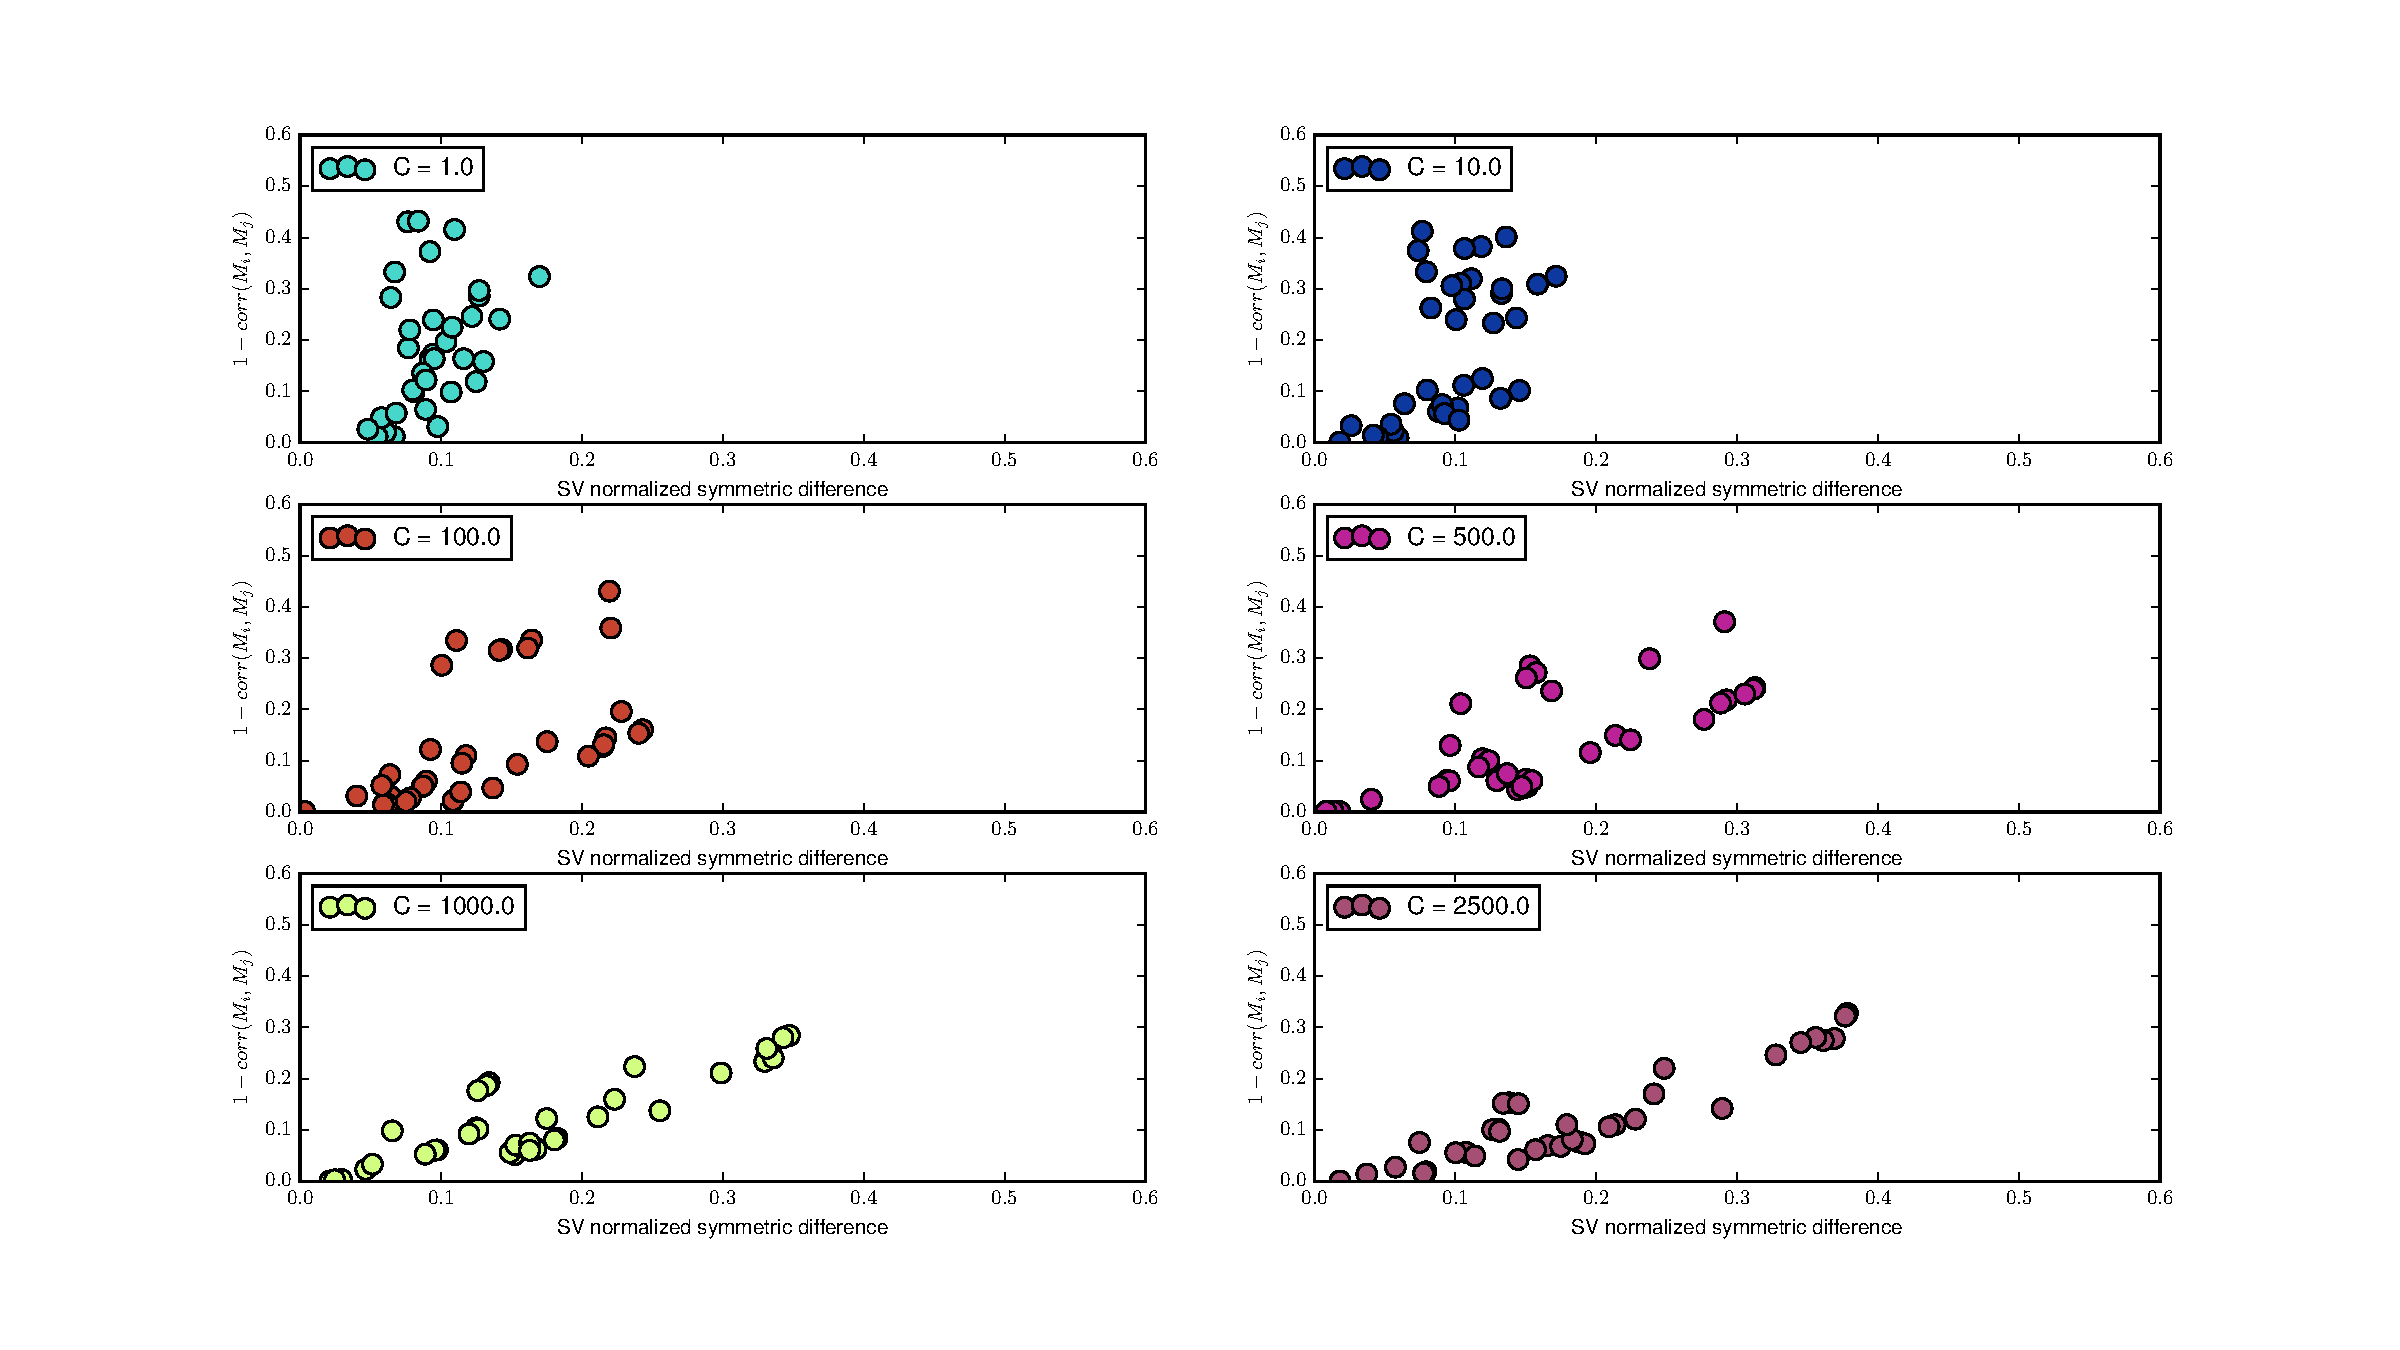
\includegraphics[width=\textwidth]{german.pdf}}
      \caption{German credit}
\end{figure}

\end{frame}

\begin{frame}{Эксперимент. German credit}
\input{german.tex_table}
\end{frame}

\begin{frame}{Эксперимент. Wine}

\begin{figure}[H]
      \center{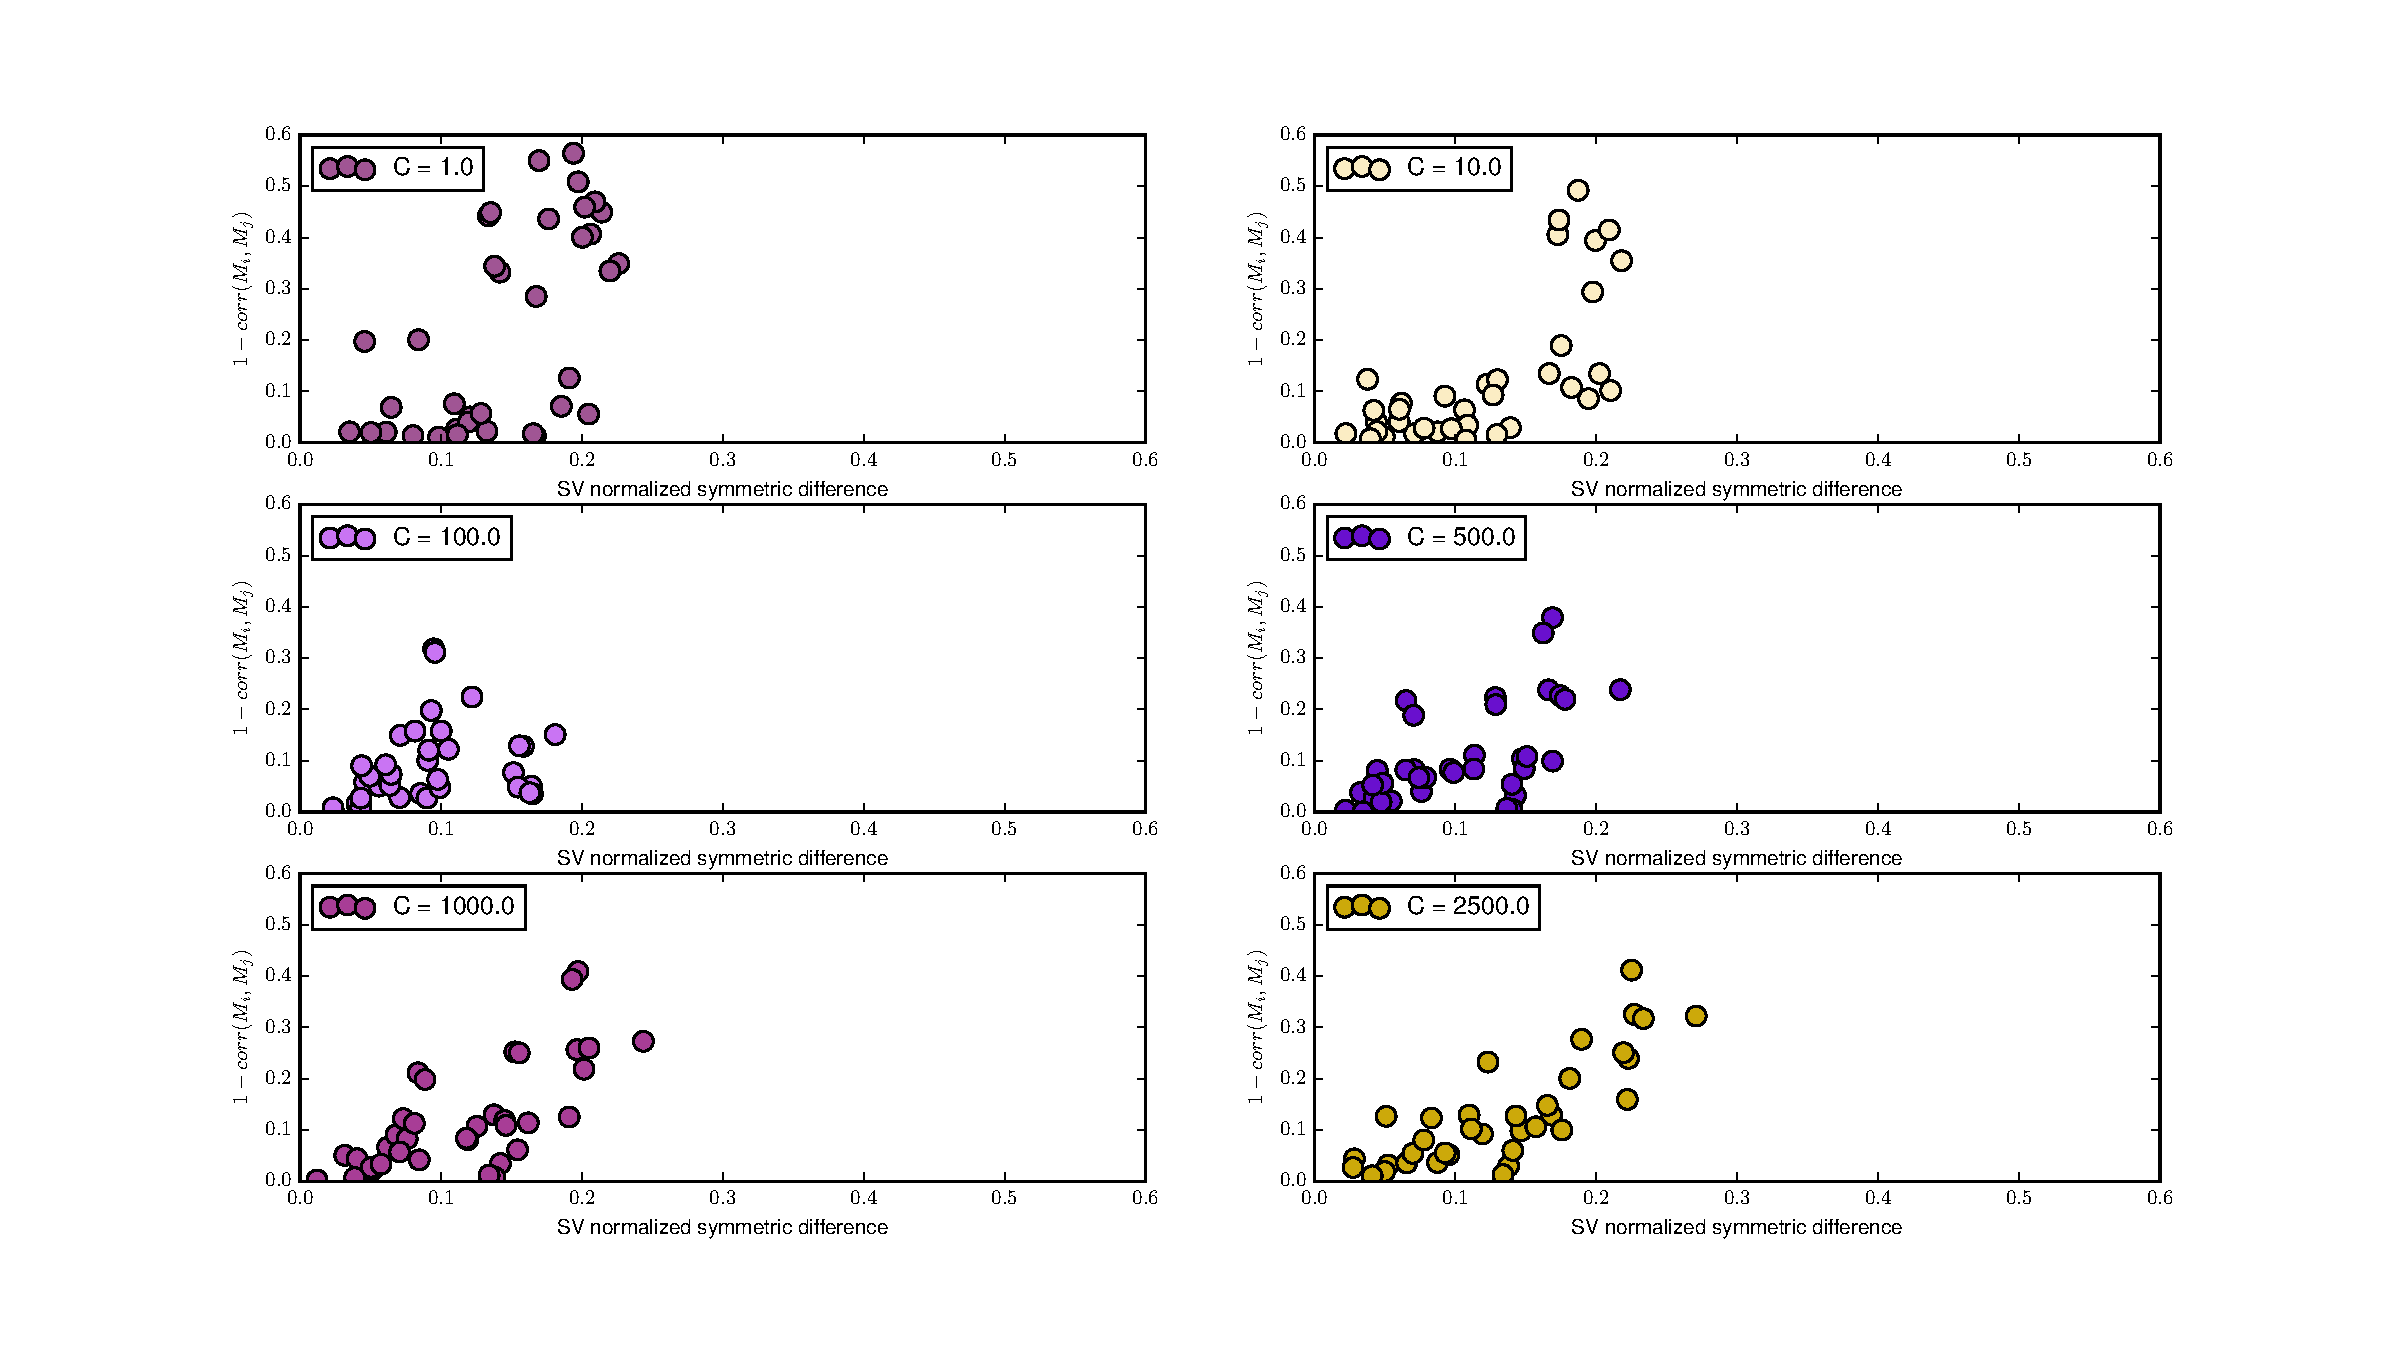
\includegraphics[width=\textwidth]{wine.pdf}}
      \caption{Wine}
\end{figure}

\end{frame}
\begin{frame}{Эксперимент. Wine}
\input{wine.tex_table}
\end{frame}
\begin{frame}{Эксперимент. Heart disease}

\begin{figure}[H]
      \center{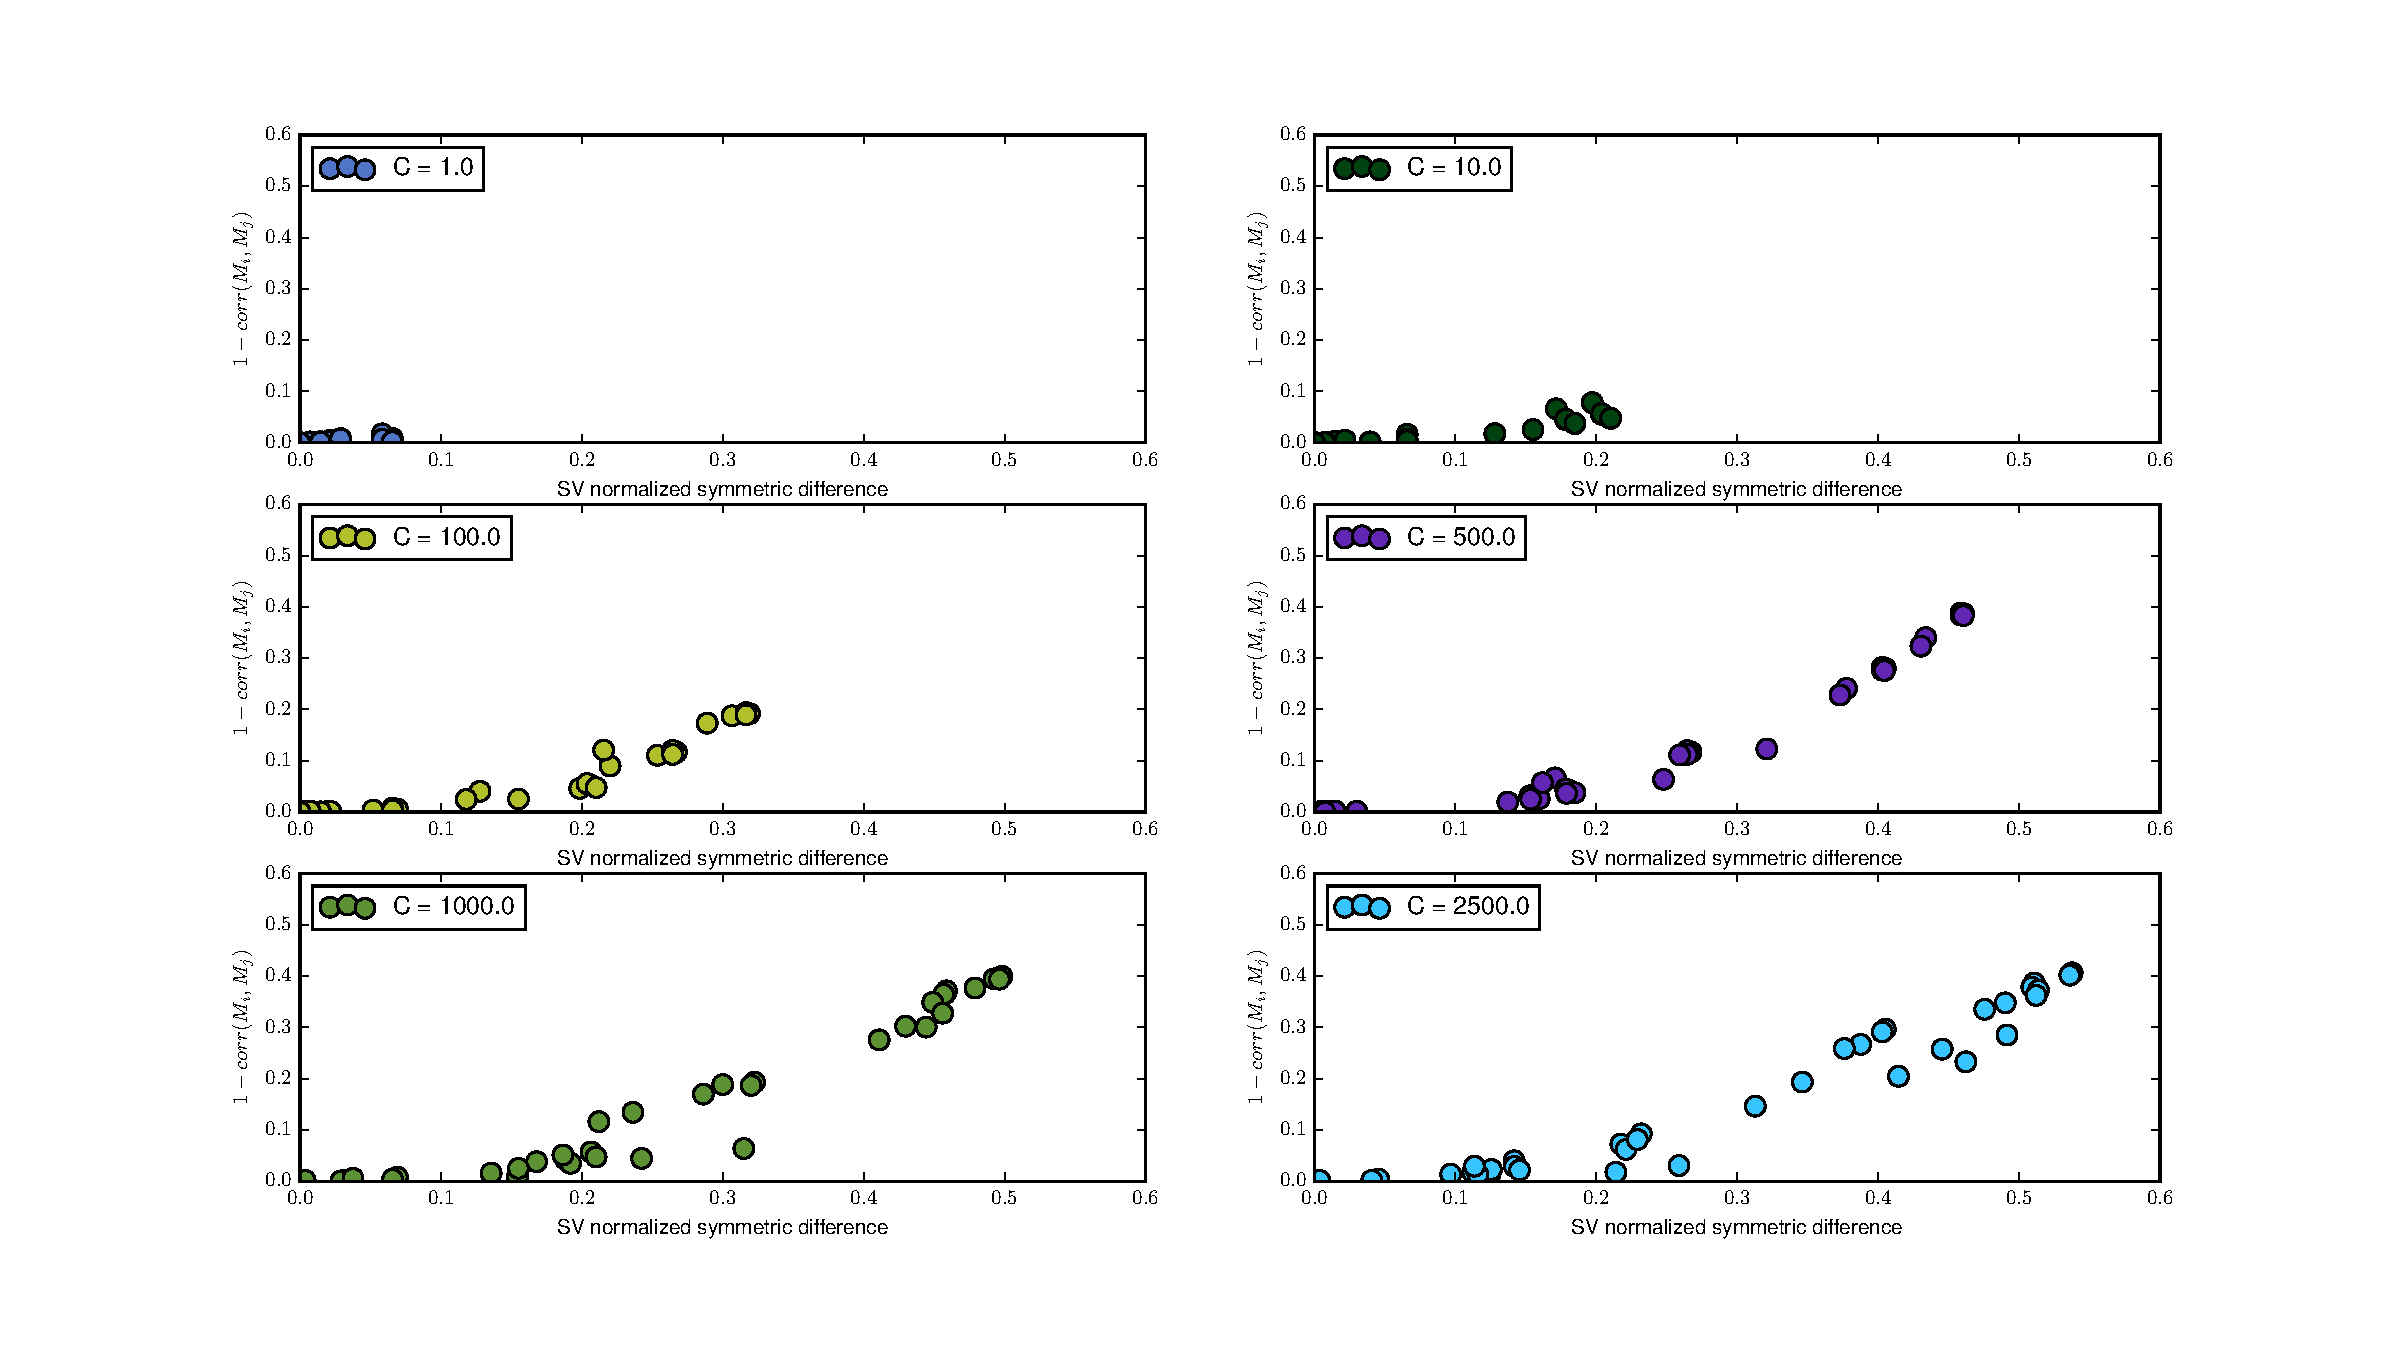
\includegraphics[width=\textwidth]{heart.pdf}}
      \caption{Heart disease}
\end{figure}

\end{frame}

\begin{frame}{Эксперимент. Heart disease}

\input{heart.tex_table}

\end{frame}
\begin{frame}{Результаты}
\begin{itemize}
  \item С ростом константы регуляризации расстояние между ядрами и расстояние между
  их отступами лучше коррелируют между собой.
  \item При высоких параметре регуляризации коэффициент корреляции Пирсона 
  достигает более $0.8$, то есть расстояния практически линейно зависят друг от друга.
  \item Вектора средних ядерных и отступных расстояний кореллируют по-разному на различных датасетах (на Wine и Heart корелляции Пирсона $0.85$ и $0.99$ соответственно, на German --- $-0.92$).
\end{itemize} 
\end{frame}

\begin{frame}{Вывод}
    Мы показали, что на примере довольно разных задач выполняется поставленная гипотеза.

    \begin{block}{Результат}
Если множества опорных объектов пары классификаторов похожи
    , то и векторы отступов похожи
    \end{block}
\end{frame}
% \begin{frame}{Построение прогноза методом авторегресии}
%     Авторегрессионная матрица целевого ряда $\mathbf{s}_1$:
%             $$
%                 \mathbf{X^*}=
%                 \left(
%                 \begin{array}{l|l}
%                 \mathbf{X}       & \mathbf{y} \\
%                 \hline
%                 \mathbf{x}_m   & x_T \\
%                 \end{array}
%                 \right).
%             $$
%     Для остальных рядов строятся матрицы $\mathbf{X}_j$ не вводя вектор $\mathbf{y}$.
%                 $$\mathbf{X}=\left[\mathbf{X}_1|\mathbf{X}_2,\ldots,\mathbf{X}_p\right].$$
%     Поставим задачу линейной регрессии: $\mathbf{y} = \mathbf{f}(\mathbf{X}\mathbf{w}) = \mathbf{X}\mathbf{w}$.\\ Тогда $x_T = \left\langle \mathbf{x}_m,\mathbf{w}\right\rangle.$
%     \begin{figure}[ht]
%       \center{\includegraphics[width=0.47\textwidth]{figs/pricesmatrix.eps}}
%       %\caption{Авторегрессионная матрица цены за четыре недели.}
%     \end{figure}
% \end{frame}
% %----------------------------------------------------------------------------------------------------------

% \begin{frame}{Отбор признаков при построении прогноза}
%     Выборка $\mathfrak{D} = (\mathbf{X}, \mathbf{y})$. Разбиение множества индексов $\mathcal{I} = \mathcal{L} \sqcup \mathcal{C}$. $\mathcal{A}$ ~--- подмножество индексов активных признаков.\\
%     Модель $\mathbf{f}_\mathcal{A}$ зависит только от множества $\mathcal{A}$.\\
%     Функция ошибки: $S = \boldsymbol{\varepsilon}^{T}\boldsymbol{\varepsilon}$, где $\boldsymbol{\varepsilon}$~--- вектор регрессионных остатков, $\boldsymbol{\varepsilon} = (\mathbf{y} - \mathbf{X}\mathbf{w})$.\\
%     Необходимо найти множество $\mathcal{A}$ минимизирующее функцию ошибки $S$ на элементах выборки $\mathfrak{D}_{\mathcal{C}}$:
%     $$\mathcal{A^*} = \argmin_{\mathcal{A} \subseteq \mathcal{J}}
%     S(\mathcal{A}|\mathbf{w^*}, \mathfrak{D_\mathcal{C}}).$$
%     Для решения этой задачи найдем вектор параметров $\mathbf{w^*}$:
%     $$\mathbf{w^*} = \argmin_{\mathbf{w} \in \mathbb{W}}
%     S(\mathbf{w}|\mathfrak{D}_\mathcal{L}, \mathcal{A}).$$
% \end{frame}

% %----------------------------------------------------------------------------------------------------------
% \begin{frame}{Метод Белсли}
%     Рассмотрим сингулярное разложение $\mathbf{X} = \mathbf{U}\mathbf{D}\mathbf{V}^T.$
%     Матрица $\mathbf{D}$ диагональная, состоит из чисел $\lambda_1 < \lambda_2 < ... < \lambda_r$. Сингулярные числа $\lambda_i$ являются собственными значениями, а столбцы матрицы $\mathbf{V}$ ~--- собственными векторами ковариационной матрицы $\hat{\mathbf{A}}^{-1}$.
%     $$\hat{\mathbf{A}}^{-1} = \mathbf{X}^{T}\mathbf{X} = \mathbf{V}\mathbf{D}^{T}\mathbf{U}^{T}\mathbf{U}\mathbf{D}\mathbf{V}^{T} = \mathbf{V}\mathbf{D}^2\mathbf{V}^{T},$$
%     $\eta_i = \lambda_{\max}/\lambda_{i}$ ~--- $i$-ый индекс обусловленности. Большое значение $\eta_i$ указывает на близкую к линейной зависимость между признаками.
%      Максимальный индекс обусловленности матрицы $\mathbf{X}$ характеризует, насколько велико будет изменение компонент вектора параметров $\mathbf{w}$ при изменении матрицы признаков $\mathbf{X}$. Назовем его \emph{числом обусловленности} $\theta$.


% \end{frame}
% %----------------------------------------------------------------------------------------------------------

% \begin{frame}{Метод Белсли}
%      Оценками дисперсии параметров будут диагональные элементы матрицы $\hat{\mathbf{A}}^{-1}$.\\
%      Дисперсионные доли $q_{ij}$ определим как вклад $j$-го признака в дисперсию $i$-го элемента вектора параметров $\mathbf{w}$:
%     $$q_{ij} = \frac{{v_{ij}}^2/{\lambda_j}^2}{\sum_{j = 1}^{n}v_{ij}^2/{\lambda_j}^2}.$$
%     Большие значения $q_{ij}$ указывают на наличие зависимости между признаками.
%     Определим индекс $j^*$, вносящий максимальный вклад в дисперсию $i$-го элемента вектора $\mathbf{w}$:
%     $$
%         j^* = \argmax_{j \in \mathcal{A}}{q_{i^*j}},\;\; \text{где}\;\; i^* = \argmax_{i \in \mathcal{A}}{\eta_i}.
%     $$
% \end{frame}
% %----------------------------------------------------------------------------------------------------------
% \begin{frame}{Метод Белсли}
%     Будем называть модель $\mathbf{f}_\mathcal{A}$ \emph{неустойчивой}, если число обусловленности матрицы признаков $\mathbf{X}$ велико: $\theta \gg 1$.
%     \begin{block}{Утверждение:}
%           Исключение из модели $\mathbf{f}_\mathcal{A}$ параметров, максимально влияющих на минимальное сингуляное значение матрицы $\mathbf{X}$ доставляет максимальную устойчивость модели.
%     \end{block}
%     \begin{figure}[ht]
%        \center{\includegraphics[width=0.5\textwidth]{figs/x1x6.eps}}
%    \end{figure}
% \end{frame}
% %----------------------------------------------------------------------------------------------------------
% \begin{frame}{Матрица Белсли}
%     \begin{table}[ht]
%     \center{\begin{tabular}{|c|c c c c c c|}
%     \hline
%     $\boldsymbol{\eta}$& $\mathbf{var}(\chi_1)$ & $\mathbf{var}(\chi_2)$ & $\mathbf{var}(\chi_3)$ & $\mathbf{var}(\chi_4)$ & $\mathbf{var}(\chi_5)$& $\mathbf{var}(\chi_6)$\\
%     \hline
%     $0$            & $0$      & $0$   & $0$ & $0$ & $0$ & $0$ \\
%     $0$            & $0$      & $0$   & $0$ & $0$ & $0$ &$0$ \\
%     $0$           & $0$      & $0$   & $0$ & $0$ & $0$ &$0$ \\
%     $1$           & $0.02$   & $0.05$   & $0$ & $0.2$ & $0.01$ &$0.53$ \\
%     $2.29$       & $0.08$   & $0.1$& $0.15$ & $0.39$ & $0.48$ &$0.23$ \\
%     $\colorbox{light-gray}{4.87}$    & \colorbox{red}{$0.9$} & \colorbox{red}{$0.85$} & $0.84$ & $0.4$ & $0.5$ & $0.24$ \\
%     \hline
%     \end{tabular}
%     }
%     \end{table}
%     \begin{figure}[ht]
%         \center{\includegraphics[width=0.5\textwidth]{figs/belsleymatrix.eps}}
%     \end{figure} \end{frame}
% %----------------------------------------------------------------------------------------------------------

% \begin{frame}{Метод отбора признаков Add-Del}
%     \begin{block}{}
%        Предполагается, что регрессионные остатки имеют нормальное распределение с нулевым матожиданием и неотрицательно определенной ковариационной матрицей. В начальный $\mathcal{A}_0 = \varnothing$.
%     \end{block}
%     Этап \textbf{Add}.
%     \begin{itemize}
%         \item Повторять:
%         \begin{itemize}
%         \item $j^* = \argmin_{j \in \mathcal{J} \backslash \mathcal{A}}
%             S(\mathbf{w}|\mathcal{A}\cup \{j\}, \mathcal{D}),$
%         \item $\mathcal{A} = \mathcal{A}\cup\{j^*\},$
%         \end{itemize}
%         \item
%         пока $S(\mathbf{w}_{\mathcal{A}}|\mathcal{D}) \geq S_{min} + \delta S_1.$\\
%     \end{itemize}
%     Этап \textbf{Del}.
%     \begin{itemize}
%     \item Повторять:
%     \begin{itemize}
%         \item $j^* = \argmax_{j \in \mathcal{A}}{q_{i^*j}},$
%             где  $i^* = \argmax_{i \in \mathcal{A}}{\eta_i}.$
%         \item $\mathcal{A} = \mathcal{A}\backslash\{j^*\},$
%     \end{itemize}
%     \item
%     пока $S(\mathbf{w}_{\mathcal{A}}|\mathcal{D}) \geq S_{min} + \delta S_2.$
%     \end{itemize}
%     Величины $\delta S_{1,2}$ определяются как дисперсия вектора регрессионных остатков $\boldsymbol{\varepsilon}$. Этапы \textbf{Add} и \textbf{Del} повторяются до тех пор, пока значение ошибки не стабилизируется.
% \end{frame}
% %----------------------------------------------------------------------------------------------------------
% \begin{frame}{Вычислительный эксперимент}
%     В ходе эксперимента сравниваются результаты прогнозирования с помощью предлагаемого метода (\emph{Add-Del} и авторегрессия) и алгоритма \emph{Гусеницы}. В качестве входных данных используются временные ряды с реальными ценами на электроэнергию в Германии
%     \begin{figure}[ht]
%       \center{\includegraphics[width=0.8\textwidth]{figs/4weeks.eps}}
%     \end{figure}
% \end{frame}
% %----------------------------------------------------------------------------------------------------------
% \begin{frame}{Авторегрессионная матрица цены за четыре недели}
%    \begin{figure}[ht]
%         \center{\includegraphics[width=\textwidth]{figs/pricesmatrix.eps}}
%     \end{figure}
% \end{frame}

% %----------------------------------------------------------------------------------------------------------

% \begin{frame}{Сравнение результатов прогнозирования}
%    \begin{figure}[ht]
%     \subfloat[]{\includegraphics[width=0.5\textwidth]{figs/AddDelforecast.eps}}
%     \subfloat[]{\includegraphics[width=0.5\textwidth]{figs/SSAforecast.eps}}
%     \caption{Сравнение прогнозируемого и реального поведения цены с использованием: a)~алгоритма Add-Del, b)~алгоритма Гусеницы.}
% \end{figure}
% Обучающая выборка содержит информацию за предшествующие $90$ дней. Время работы алгоритмов практически одинаково.
% \end{frame}
% %----------------------------------------------------------------------------------------------------------
% \begin{frame}{Сравнение качества построенных моделей}

% \begin{figure}[ht]
%     \center{\includegraphics[width=\textwidth]{figs/comparison_all.eps}}
% \end{figure}
% \begin{table}[th]
%     \center{\begin{tabular}{|c|c|c|c|c|}
%     \hline
%      & RSS & AIC & BIC & Число \\
%      & & & &признаков, $n$\\
%     \hline
%     Add-Del& 57.97 & 237.97 & 343.99  & 11\\
%         \hline
%      LARS & 0.82 & 178.82 & 283.67 & 23\\
%     \hline
%     Lasso& 104.01 & 282.01 & 386.86 & 18\\
%     \hline
%     \end{tabular}}
% \end{table}
% \end{frame}
% %----------------------------------------------------------------------------------------------------------
% \begin{frame} {Заключение}
%     \begin{block} {Выводы:}
%     \begin{itemize}
%         \item Предложенный подход к проблеме мультиколлинеарности применим и позволяет обнаруживать и устранять мультикоррелирующие признаки.
%      \item Примененимость данного метода в рамках задачи прогнозирования обоснована и проверена на практике.
%     \end{itemize}
%     \end{block}
%     \begin{block} {Идеи для дальнейшей работы:}
%      Найти способ обнаружения нелинейных зависимостей между признаками.
%     \end{block}
% \end{frame}

%----------------------------------------------------------------------------------------------------------
\end{document} 
